\documentclass{article}
\usepackage[margin=0.80in, a4paper]{geometry} % Adjust margins here
\usepackage{amsmath}
\usepackage{float}
\usepackage{url} % For formatting URLs
\usepackage{hyperref}
\usepackage{subcaption}
\usepackage{graphicx} % subcaption for subfigure environment
\graphicspath{{./img/}}
%%%%%%%%%%%%%%%%%%%%%%%%%%%%%%%%%%%%%%%%%%%%%%%%%%%%%%%%%%%%%%%%%
\author{Francesco Sermi\\Francesco Angelo Fabiano Antonacci}

\date{\today}
\title{Relazione FFT}
%%%%%%%%%%%%%%%%%%%%%%%%%%%%%%%%%%%%%%%%%%%%%%%%%%%%%%%%%%%%%%%%%

\begin{document}
\maketitle

\section{Forme d'onda sinusoidali}

\section{Forme d'onda quadrate}

\section{Forme d'onda triangolari}

\section{Forme d'onda treni di impulsi}

\section{Forme d'onda pinne di squalo}

\section{Forme d'onda acquisite male}

\section{Forme d'onda col duty cycle}

\section{Autoscillatore}

Sono state prese delle misure di un segnale in uscita da un autoscillatore, il cui schema è riportato in Fig(\ref{fig:circuitino_oscillante})
\begin{figure}[H]
    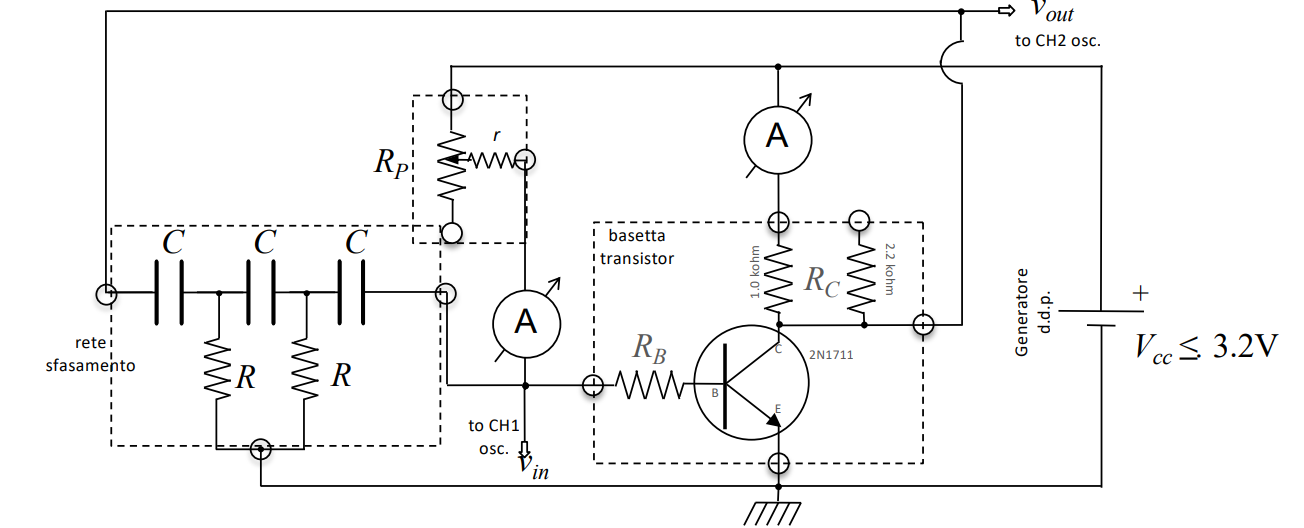
\includegraphics[scale=0.50]{FFT11/schema_circuitino.png}
    \caption{Schema circuitale dell'oscillatore}
    \label{fig:circuitino_oscillante}
\end{figure}
E' stato eseguito il fit ai minimi quadratici per individuare la frequenza dell'oscillazione sinusoidale del segnale in uscita, confrontandolo con il contenuto spettrale ottenuto tramite l'algoritmo della RFFT.
Riportiamo in Fig() i grafici con a sinistra il segnale in uscita e a destra la trasformata del segnale
\begin{figure}[H]
    \centering
    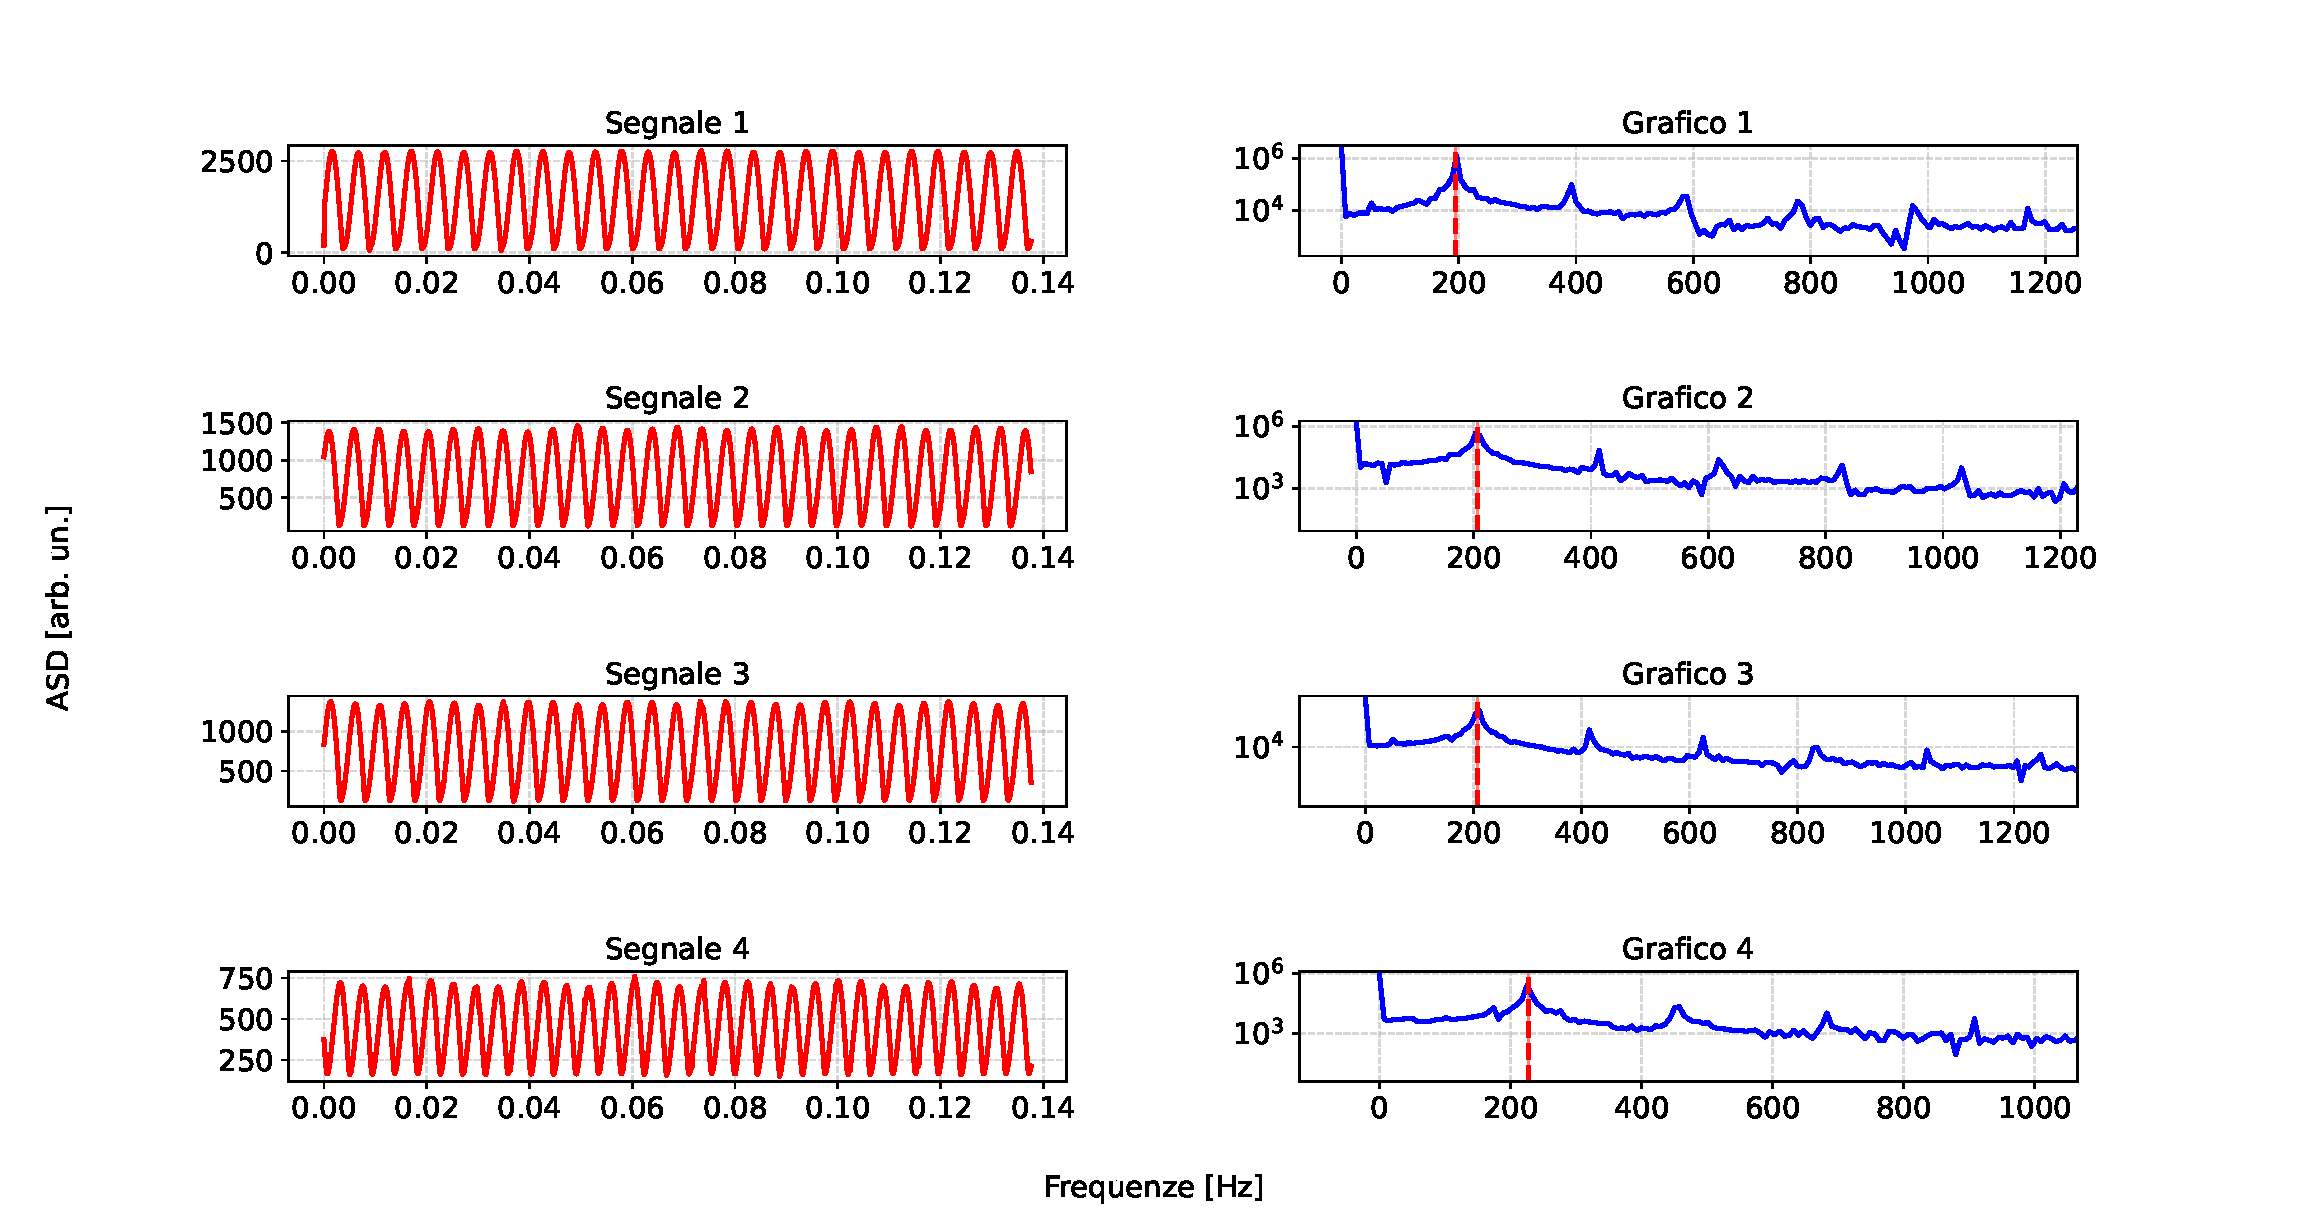
\includegraphics[width=\textwidth]{FFT11/first_graph.pdf}
    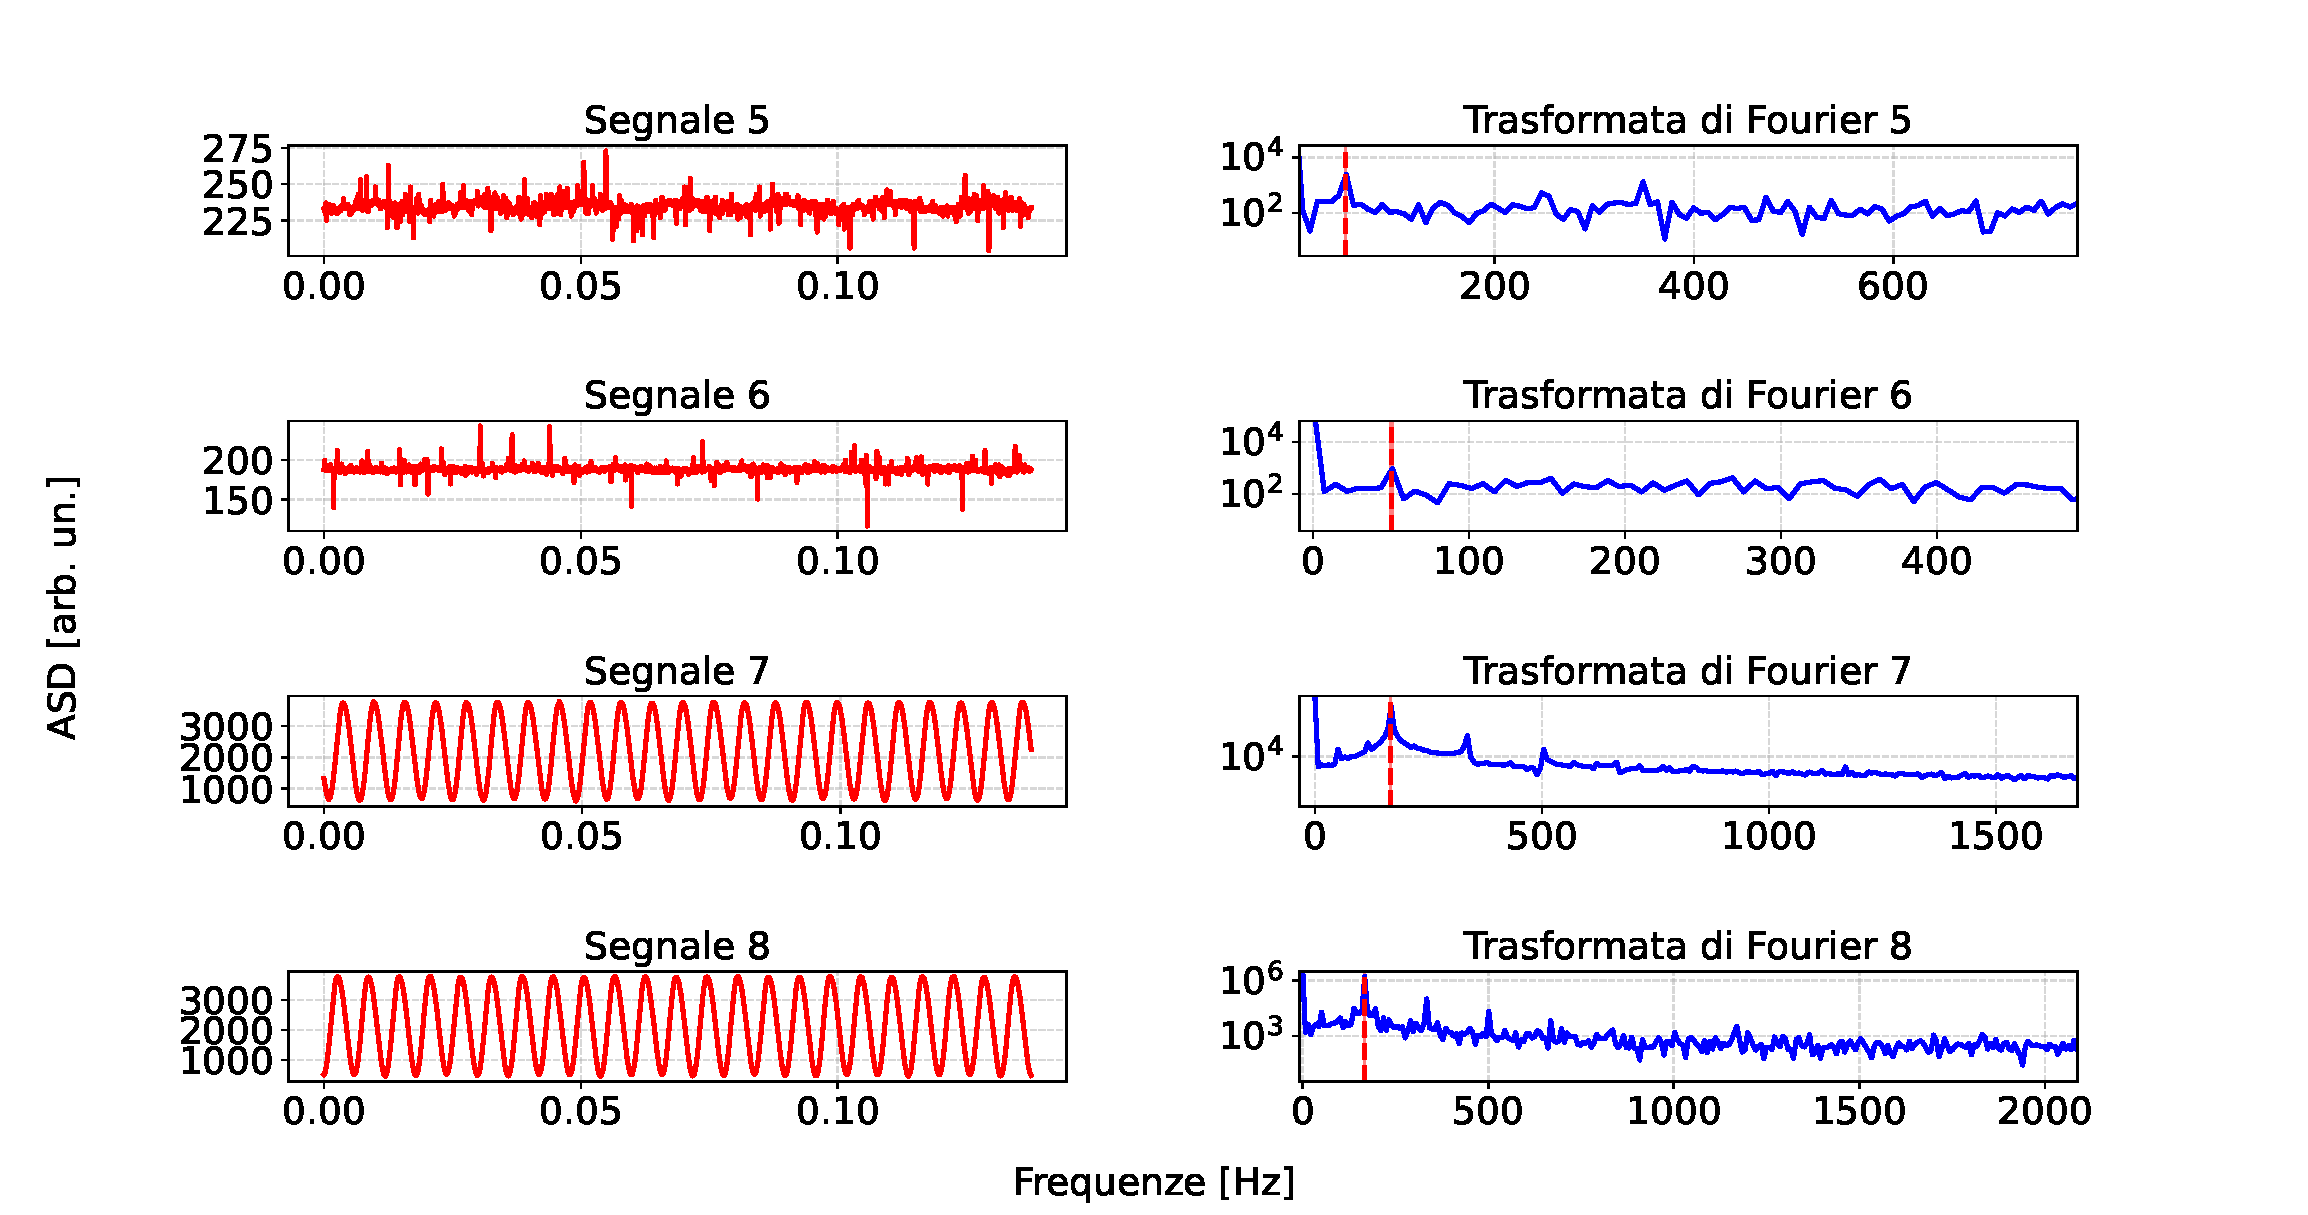
\includegraphics[width=\textwidth]{FFT11/second_graph.pdf}
    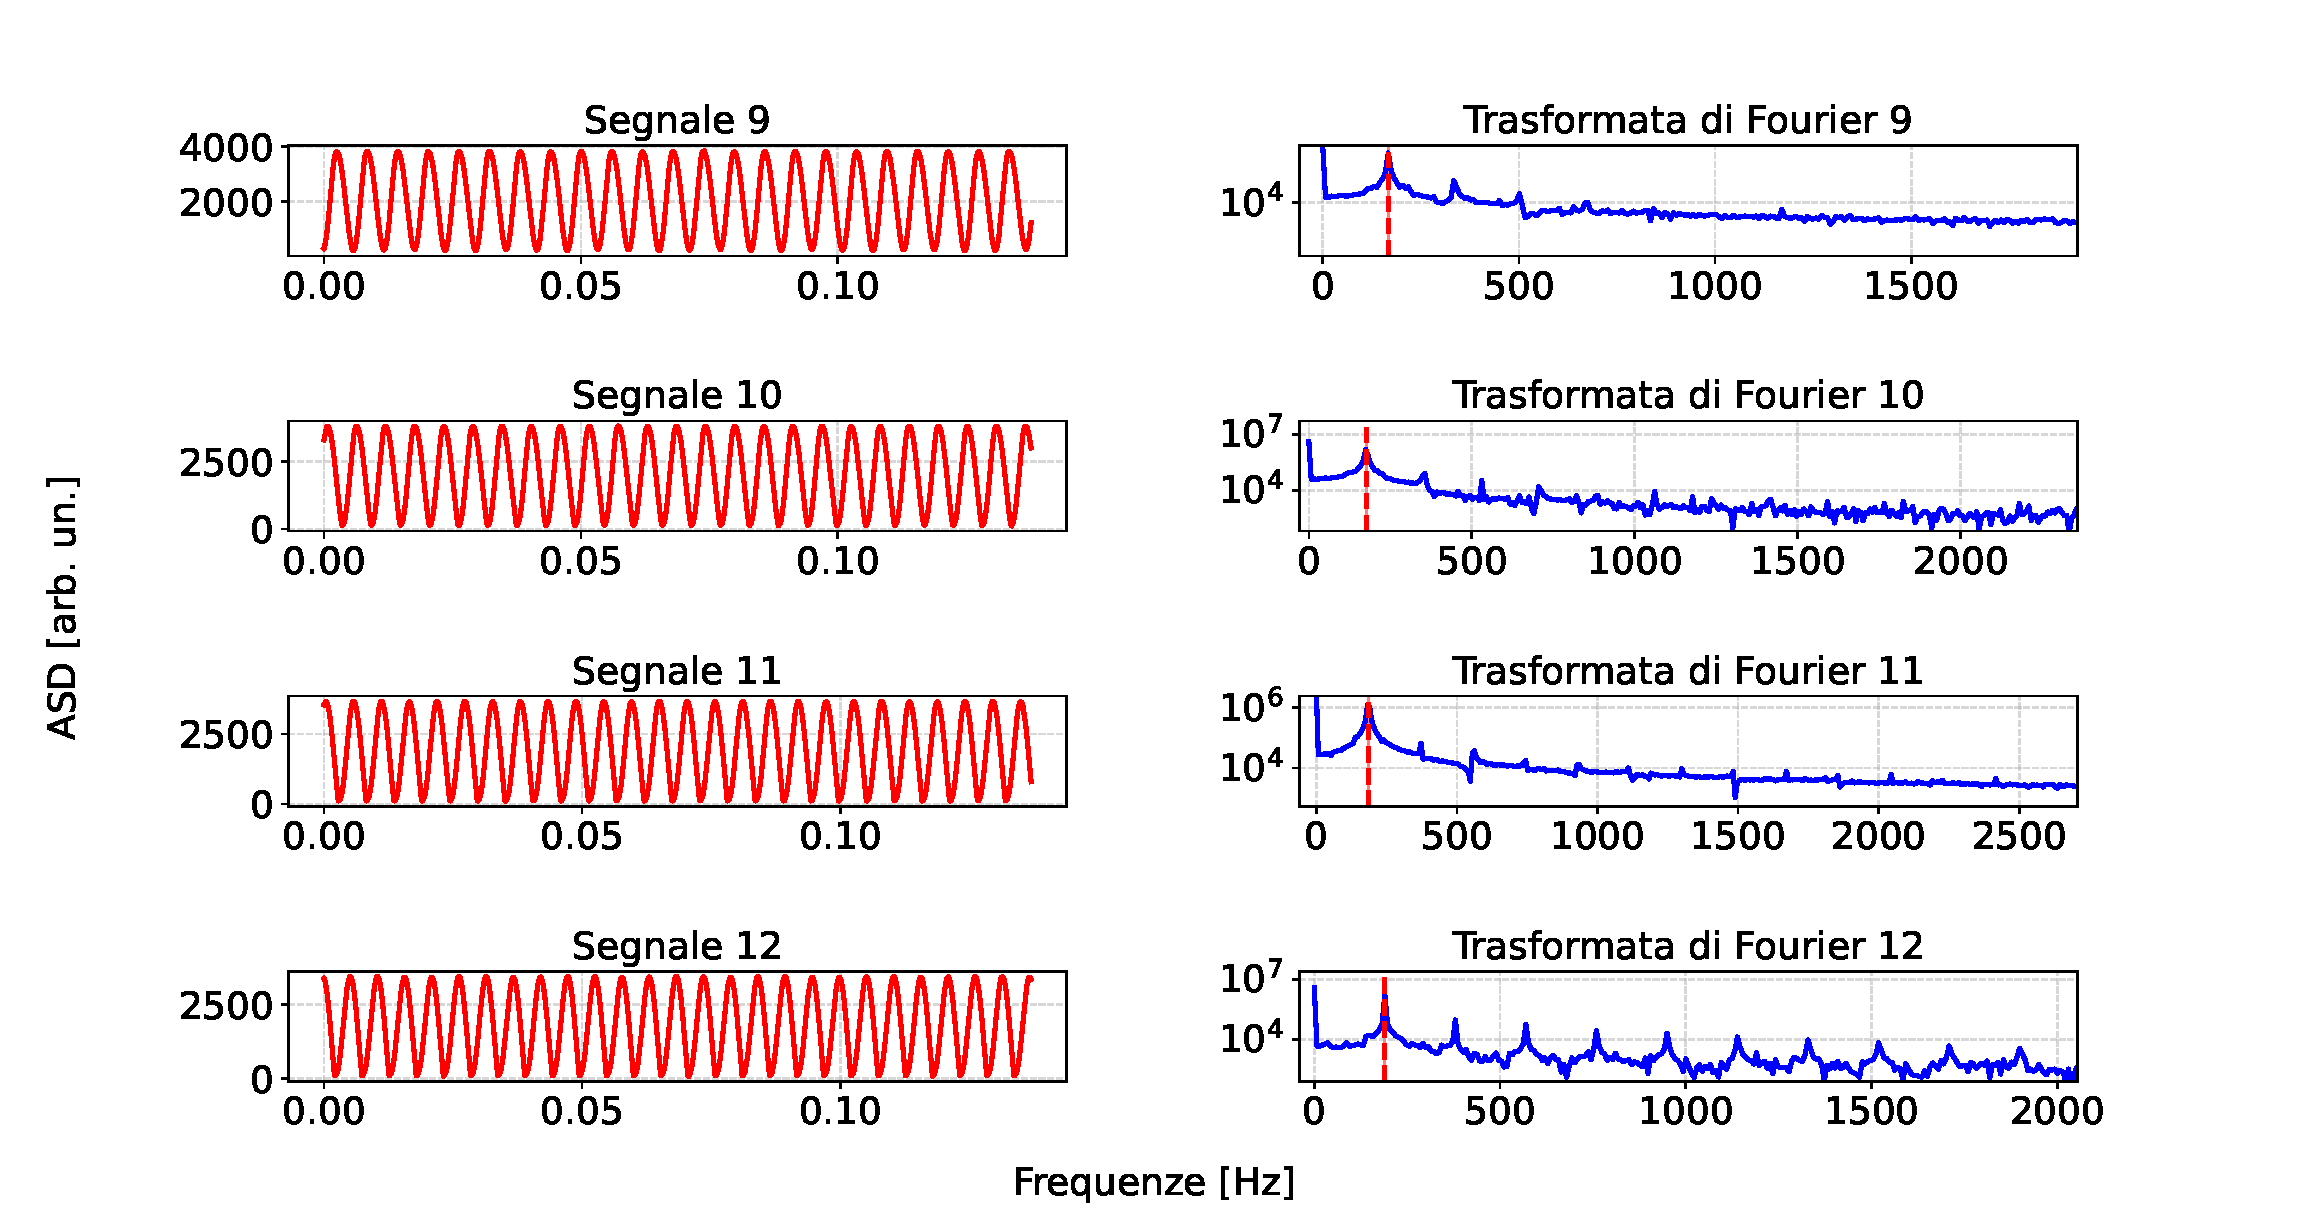
\includegraphics[width=\textwidth]{FFT11/third_graph.pdf}
    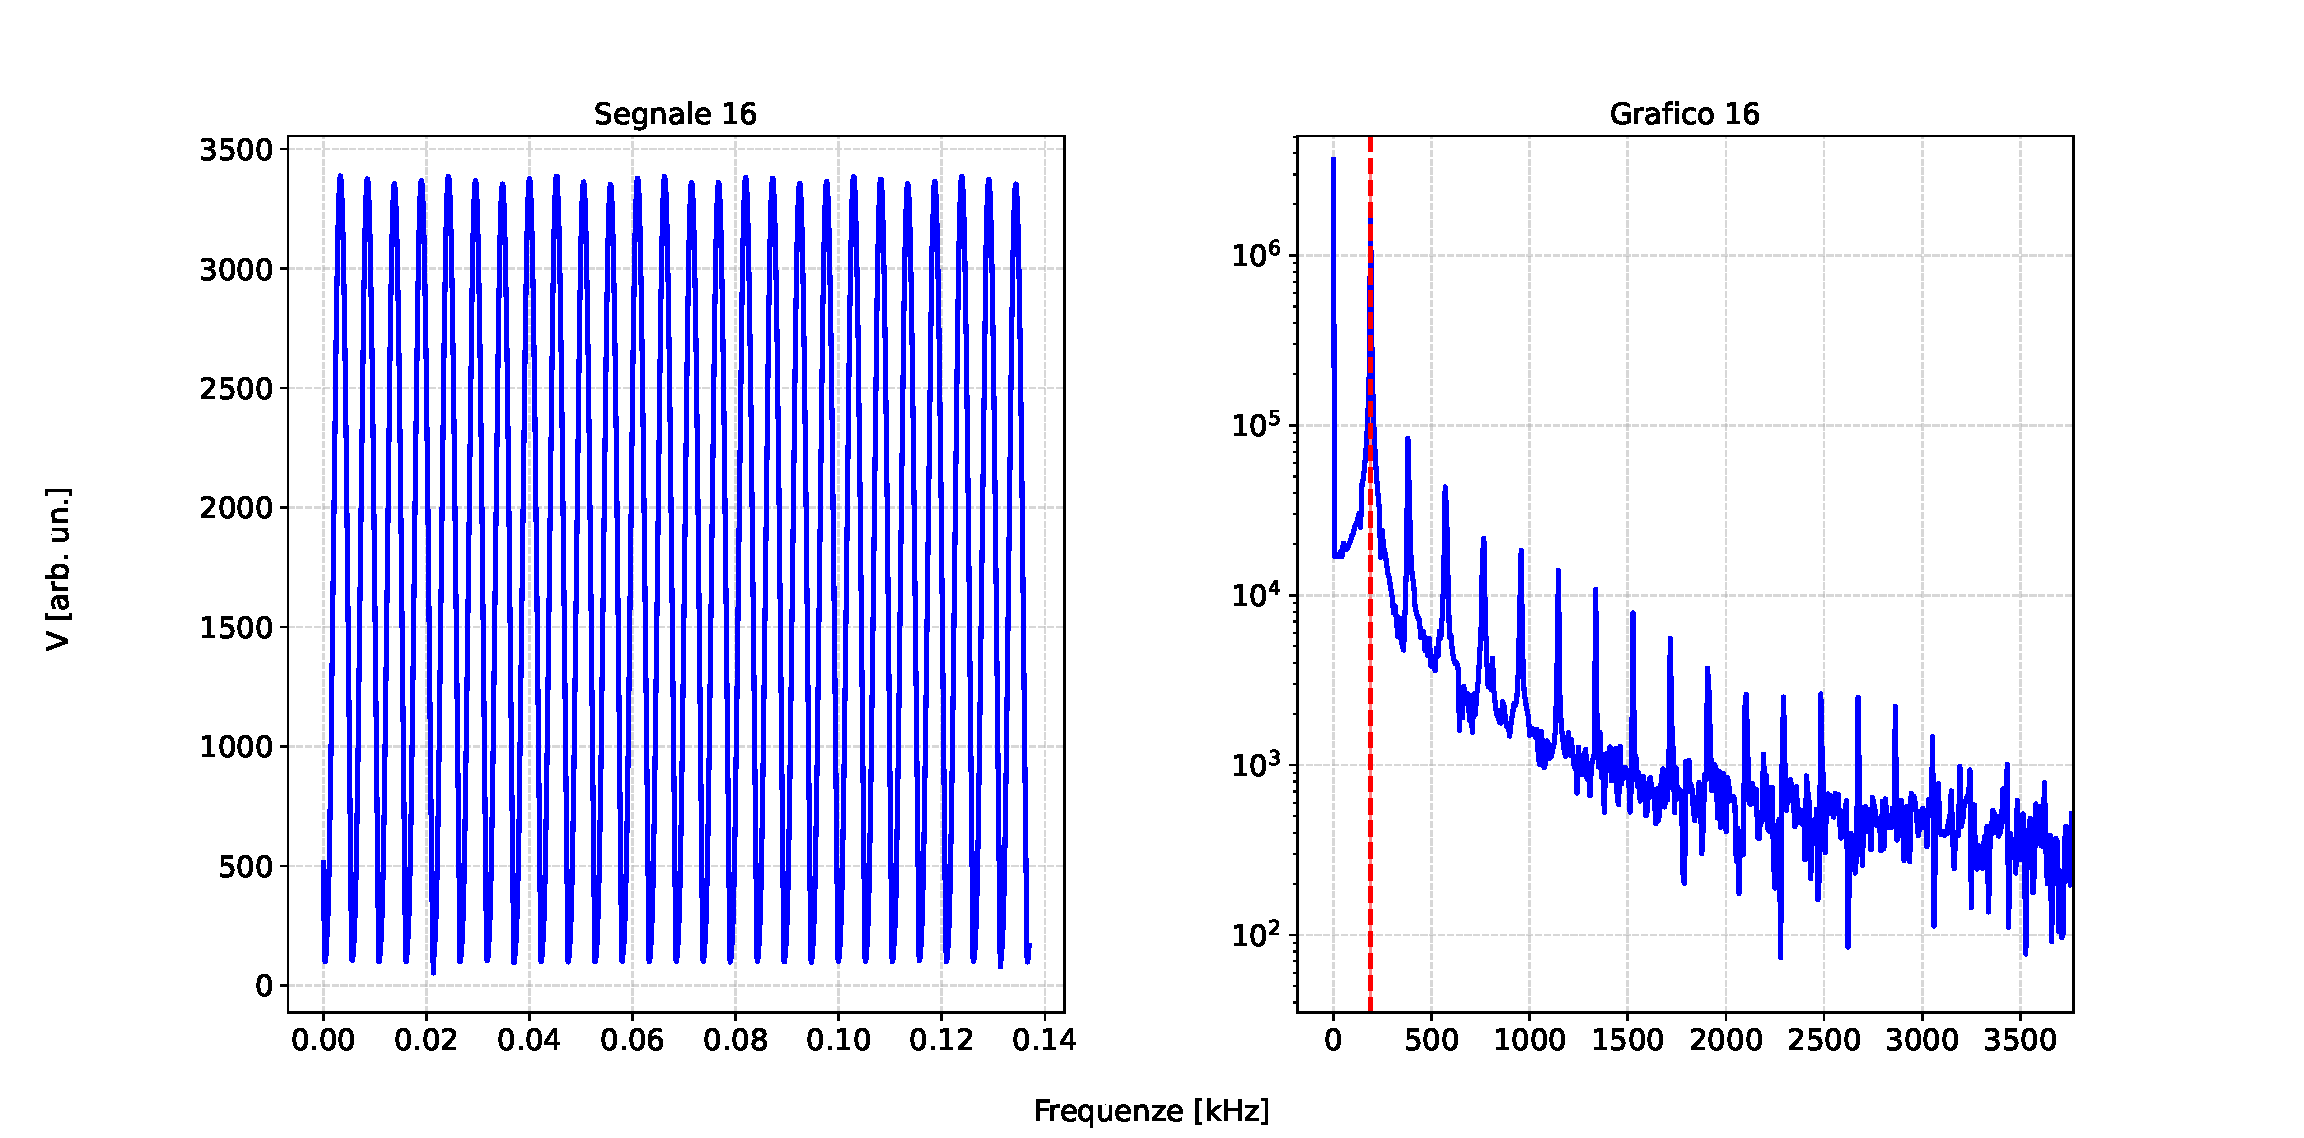
\includegraphics[width=\textwidth]{FFT11/fourth_graph.pdf}
\end{figure}

\section{Oscillazioni smorzate}

        
        \begin{figure}[H]
            \begin{minipage}{0.45\textwidth}
                Sono state prese delle misure di segnale in uscita da un circuito RLC,
                come mostrato in Fig($\ref{fig:osc_diag}$) per tre diversi condensatori.
                Sono stati misurati il periodo e la frequenza delle oscillazioni.
                E' stato eseguito un fit ai minimi quadrati per un'oscillazione 
                smorzata per determinarne il periodo.
                E' stata eseguita una FFT per il medesimo scopo.
                I risultati sono riportati in Tab.($\ref{tab:osc_smor}$) e 
                in Fig.($\ref{fig:osc_smor}$).
            \end{minipage}%
            \hfill
            \begin{minipage}{0.45\textwidth}
                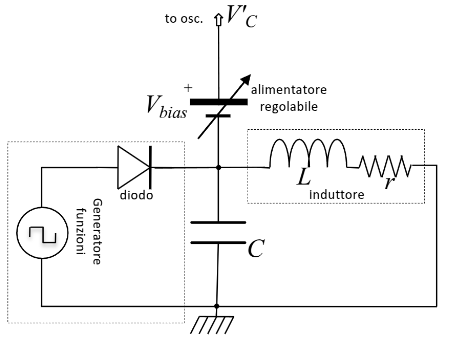
\includegraphics[width=\textwidth]{FFT12/RLCdiagram.png}
                \caption{Diagramma del circuito RLC realizzato.}
                \label{fig:osc_diag}
            \end{minipage}
        \end{figure}

        \begin{figure}[H]
            \centering
            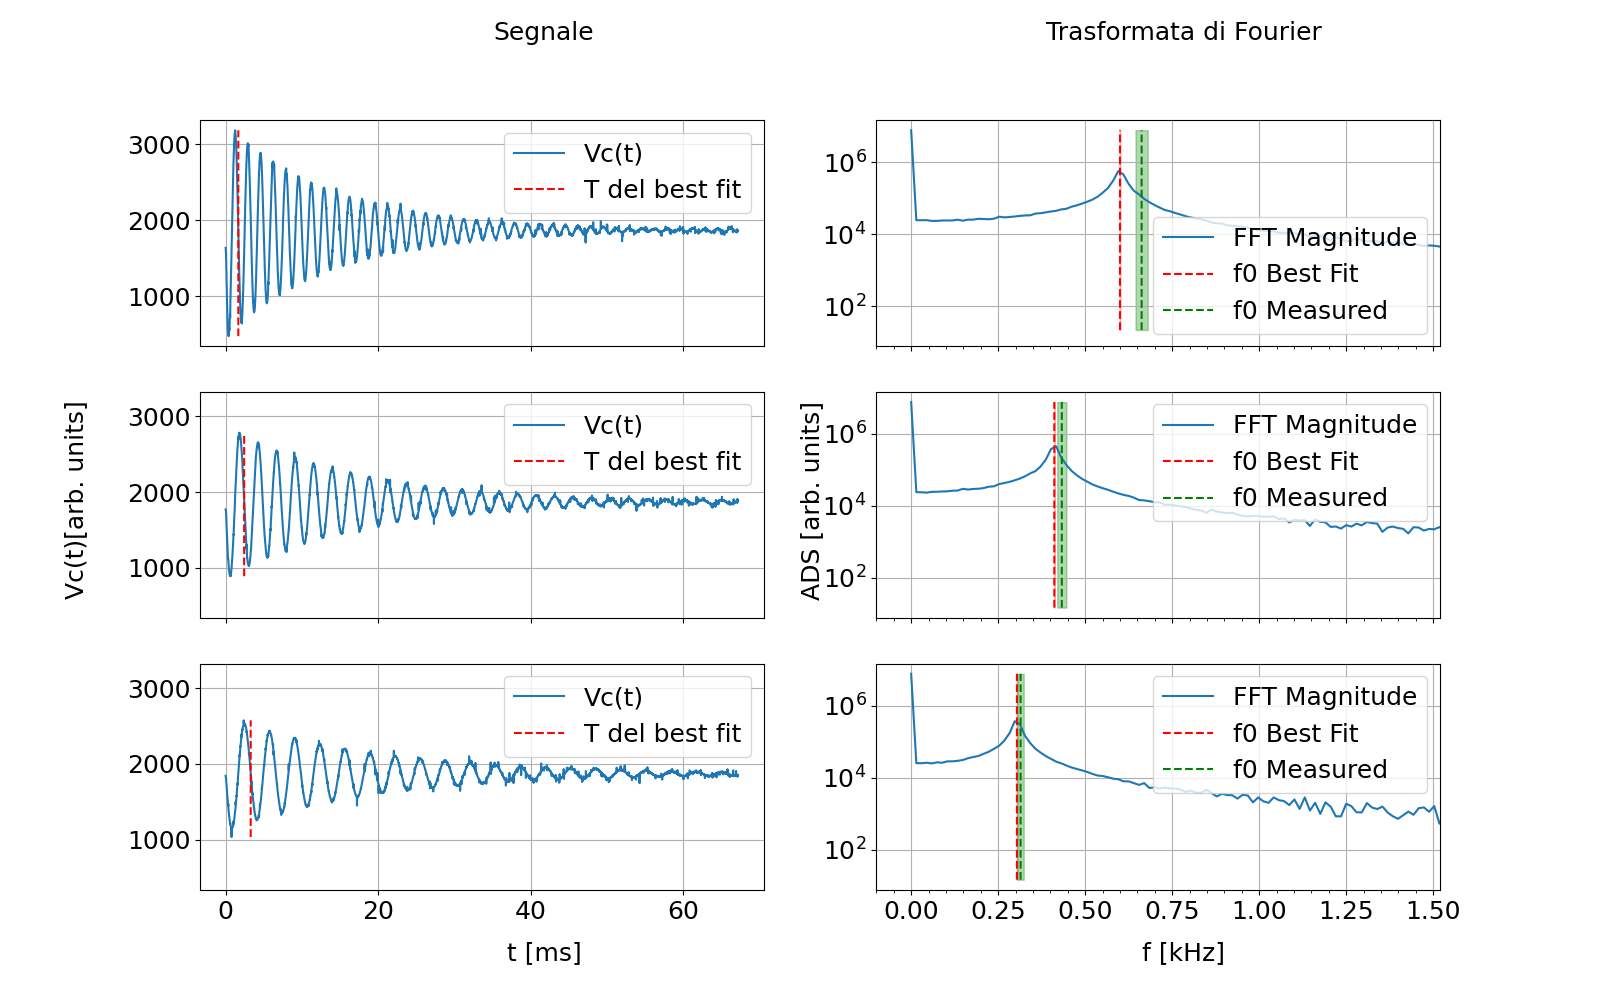
\includegraphics[width=\textwidth]{FFT12/FFTRLC.png}
            \caption{}
            \label{fig:osc_smor}
        \end{figure}

        \begin{table}[H]
            \centering
            \caption{Confronto tra le frequenze di oscillazione misurate con quelle ottenute tramite FFT e bestfit.
                    Attorno ai valori medi è stata rappresentata la barra di errore per il valore
                    misurato e per quello del bestfit, per il quale non si vede essendo molto piccola.}
                \begin{tabular}{cccc}
                    $C$[$\mu$F]          &$f_{0mis}$                &   $f_{0fft}$[kHz]       & $f_{0bestfit}$[kHz] \\
                    \hline
                    $0.1 \pm 20\%tol.$   &     $0.66 \pm 0.02$      & $0.595 \pm 0.004$       & $0.6001 \pm 0.0003$ \\
                    $0.22 \pm 20\%tol.$  &$0.43 \pm 0.01$           & $0.416 \pm 0.004$       & $0.41131\pm 0.00002$ \\
                    $0.47 \pm 20\%tol.$  &$0.314 \pm 0.009 $        &$0.298 \pm 0.004$        & $0.30393\pm 0.00002$ \\
                \end{tabular}
                \label{tab:osc_smor}

        \end{table}
    
    Le frequenze ottenute tramite la FFT e tramite il bestfit sono compatibili, 
    eccetto per la prima frequenza misurata, entro la barra di errore.

    Coerentemente con quanto ci si può aspettare sono presenti 2 picchi nella FFT,
    uno a frequenza nulla, in quanto il segnale non è alternato, l'altro
    alla frequenza di oscillazione del segnale.

    Siccome il segnale non è perfettamente sinusoidale, la FFT
    presenta un ampio spettro di armoniche attorno al picco principale.

\section{Materiali nel core dell'induttore}
\begin{figure}[H]
    \begin{minipage}{0.45\textwidth}
        Sono state prese delle misure di segnale in uscita da un circuito RLC,
        come mostrato in Fig($\ref{fig:mat_diag}$) inserendo diversi materiali dentro 
        il core dell'induttore.
        E' stato eseguito un fit ai minimi quadrati per un'oscillazione 
        smorzata per determinarne il periodo e il tempo di smorzamento.
        E' stata eseguita una FFT per determinare il periodo di oscillazione.
        I risultati sono riportati in Tab.($\ref{tab:mat_smor}$) e 
        in Fig.($\ref{fig:mat_smor}$).
    \end{minipage}
    \hfill
    \begin{minipage}{0.45\textwidth}
        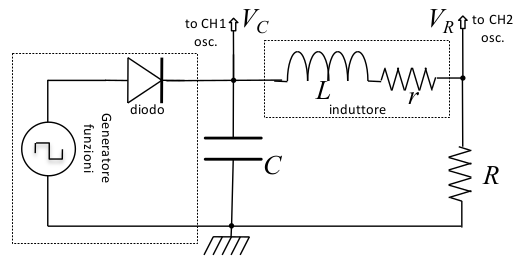
\includegraphics[width=\textwidth]{FFT13/RLCmaterialsdiagram.png}
        \caption{Diagramma del circuito RLC realizzato.}
        \label{fig:mat_diag}
    \end{minipage}
\end{figure}

        \begin{figure}[H]
            \centering
            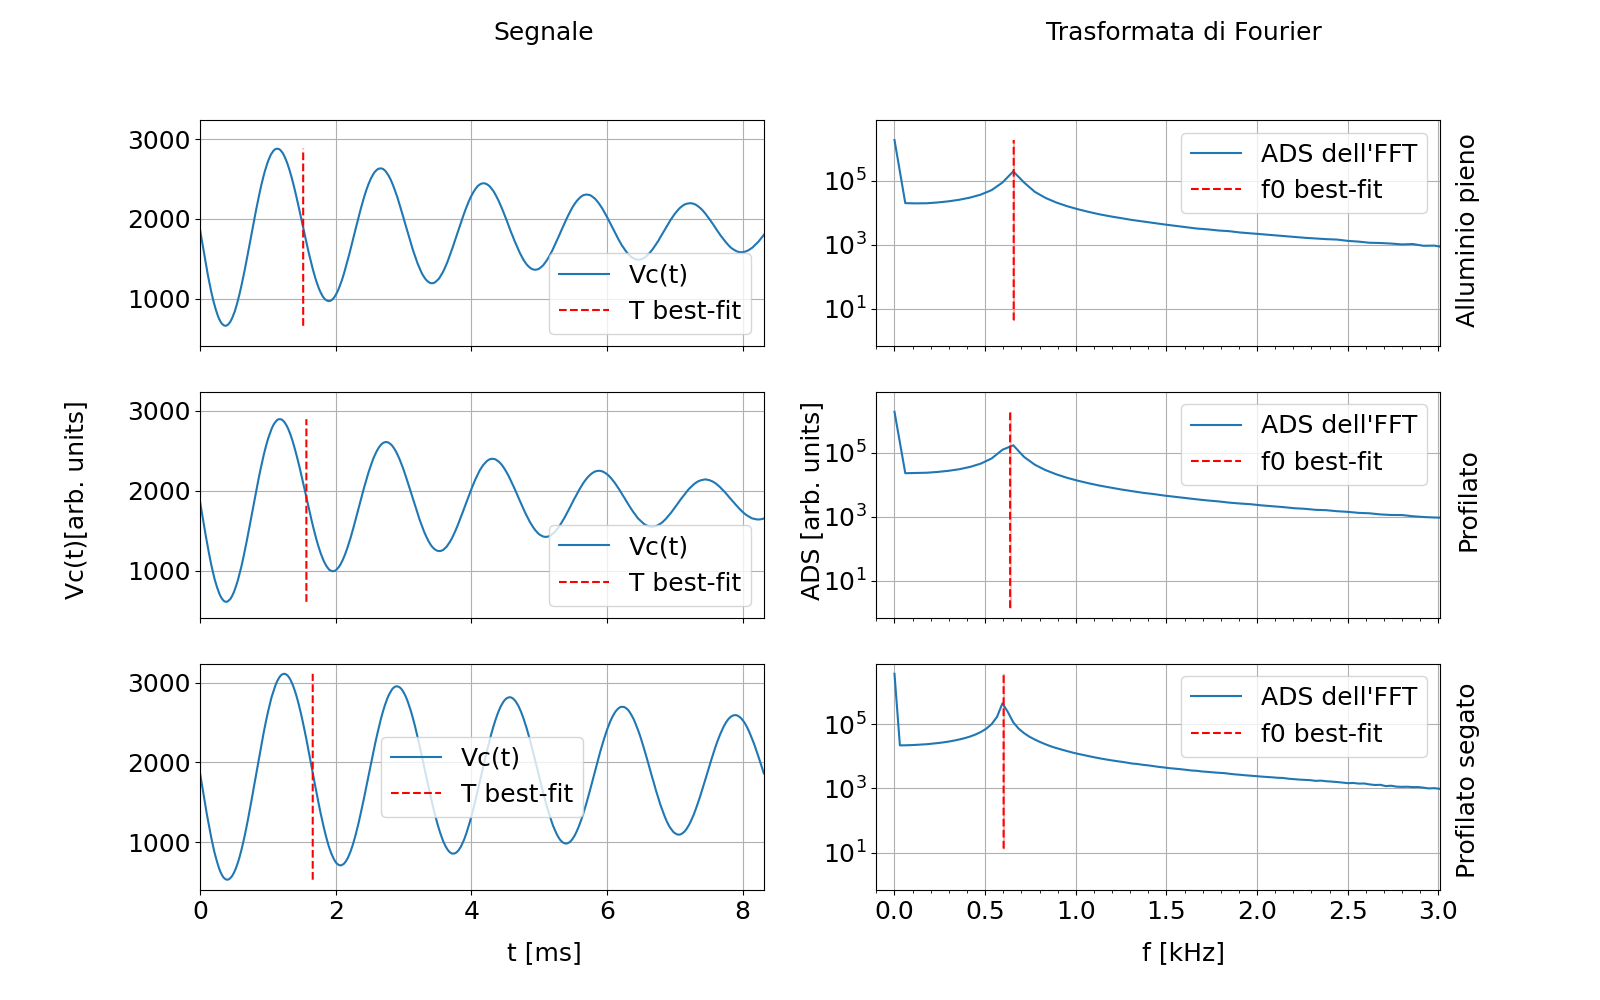
\includegraphics[width=\textwidth]{FFT13/FFTMATERIALS1.png}
            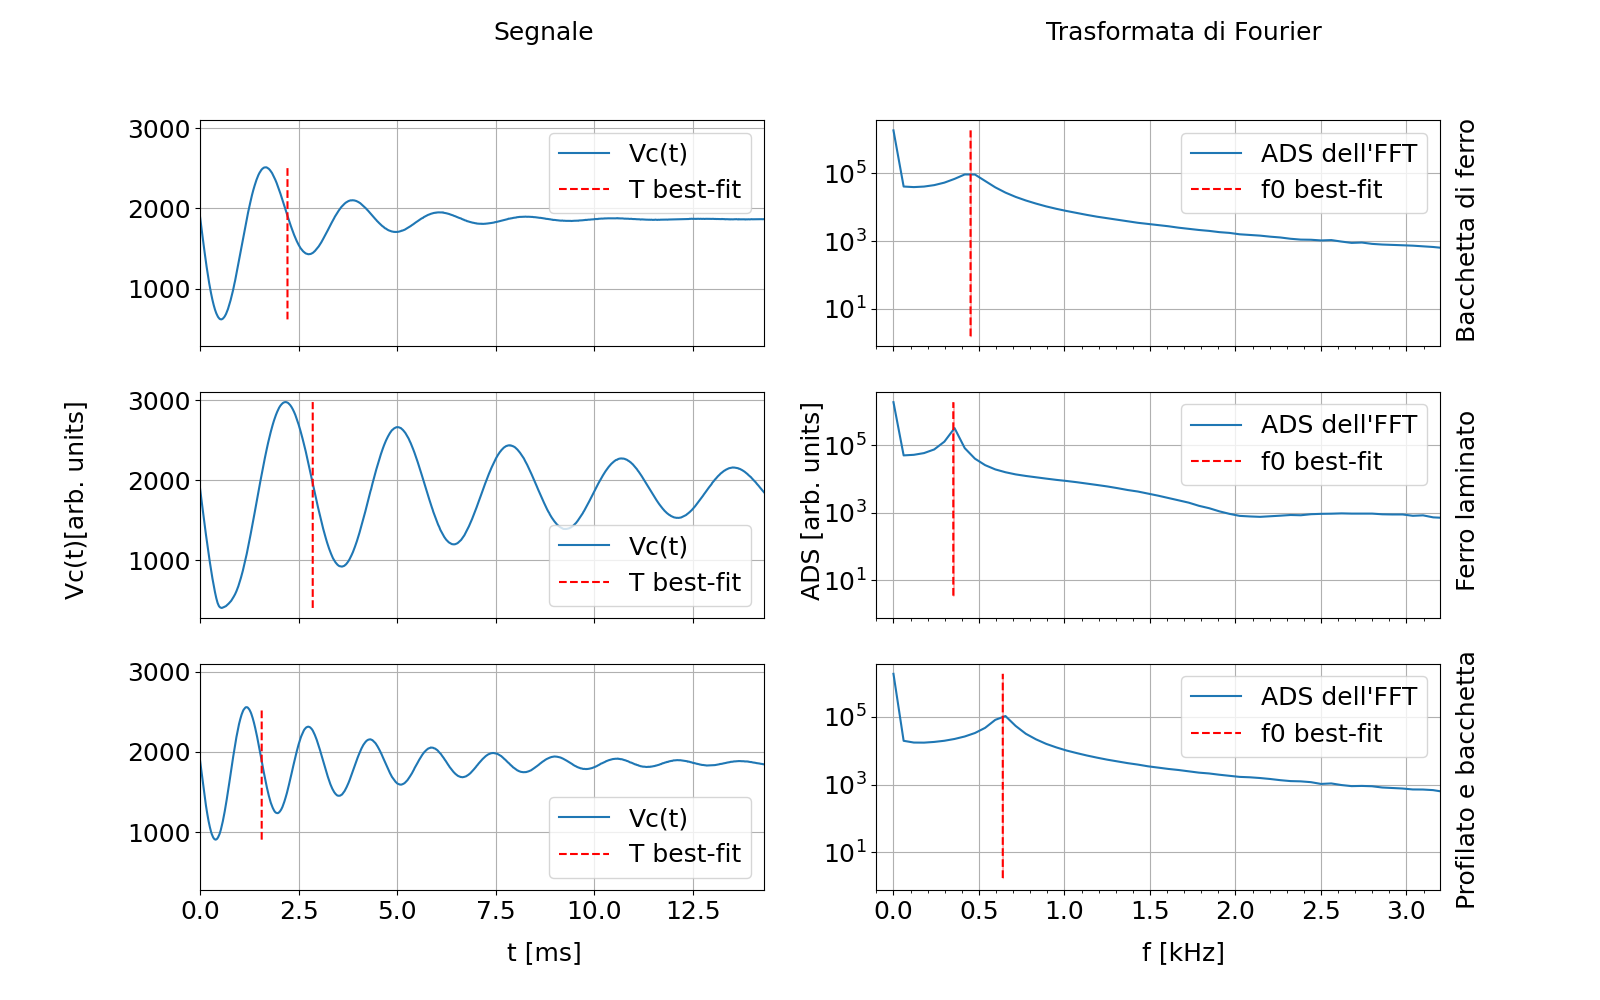
\includegraphics[width=\textwidth]{FFT13/FFTMATERIALS2.png}
            \caption{Confronto tra le frequenze di oscillazione misurate con quelle ottenute tramite FFT e bestfit.
            Attorno ai valori medi è stata rappresentata la barra di errore per il valore
            misurato e per quello del bestfit, per il quale non si vede essendo molto piccola.}
            \label{fig:mat_smor}
        \end{figure}

        \begin{table}[H]
            \centering
            \caption{Confronto tra le frequenze di oscillazione misurate con quelle ottenute tramite FFT e bestfit.
                    Attorno ai valori medi è stata rappresentata la barra di errore per il valore
                    misurato e per quello del bestfit, per il quale non si vede essendo molto piccola.}
                \begin{tabular}{ccc}
                    materiale           &   $f_{0fft}$[kHz]     & $f_{0bestfit}$[kHz] \\
                    \hline
                    Alluminio pieno     & $0.65\pm0.02$         & $0.65742\pm0.00008$ \\
                    Profilato           & $0.65\pm0.02$         & $0.63773\pm0.00008$ \\
                    Profilato segato    & $0.595\pm0.009$       & $0.60181\pm0.00002$ \\
                    Bacchetta di ferro  & $0.42\pm0.02$         & $0.4509\pm0.0002$ \\
                    Ferro laminato      & $0.35\pm0.02$         & $0.34989\pm0.0006$ \\
                    Profilato e bacchetta& $0.65\pm0.02$        & $0.6393\pm0.0002$ \\  
                \end{tabular}
                \label{tab:mat_smor}

        \end{table}

        Le frequenze ottenute tramite la FFT e tramite il bestfit sono compatibili, 
        eccetto per la bacchetta di ferro, entro la barra di errore.
        Il problema con la bacchetta di ferro è che essendo il segnale molto smorzato 
        e il picco non è molto pronunciato; in aggiunta siccome l'acquisizione non è stato
        possibile prenderla suffiecienemente lunga -in quanto il segnale sarebbe stato 
        eccessivamente soppresso-, si sovrappone al problema precedente 
        uno legato alla scarsa risoluzione dei punti nello spettro delle frequenze.

        
        Si può osservare che per i blocchi di alluminio pieno e profilato di alluminio,
        il periodo di oscillazione diminuisce, in quanto è diamagnetico e il periodo
        è inversamente proporzionale all'induttanza,che diminuisce.
        
        Analogamente per il ferro laminato e ,in maggior misura, per la bacchetta di 
        ferro il periodo di oscillazione aumenta per il comportamento da ferromagnete.
        
        Nella discussione appena fatta sto trascurando il contributo dato dal 
        tempo caratterstico di smorzamento al periodo di oscillazione.
        
        Il tempo caratteristico di smorzamento è rilevante nei grafici 
        delle FFT, Fig($\ref{fig:mat_smor}$), in quanto impone l'ampiezza del picco:
        si osserva che questo aumenta per ogni materiale inserito nel core 
        rispetto a quanto visto nel caso  del vuoto visto a Fig.($\ref{fig:osc_smor}$).
        Tuttavia questo non accade per il profilato segato dove, è possibile  
        aspettarsi che gli effetti delle correnti parassite siano meno importanti.

        

\section{Glicemia}

\section{"Il pinnacolone"}

\end{document}